
\documentclass[journal]{IEEEtran}

\usepackage{amsmath, amsthm, amssymb, amsfonts}
\usepackage{graphicx}
\usepackage[colorlinks=true,linkcolor=red, citecolor=red]{hyperref}
% \usepackage{algorithm}
% \usepackage{algpseudocode}
% \usepackage{minted}
\usepackage{booktabs}

% decrease table's cells left and right padding
\setlength{\tabcolsep}{5pt}


% correct bad hyphenation here
\hyphenation{op-tical net-works semi-conduc-tor}


\begin{document}
%
% paper title
% Titles are generally capitalized except for words such as a, an, and, as,
% at, but, by, for, in, nor, of, on, or, the, to and up, which are usually
% not capitalized unless they are the first or last word of the title.
% Linebreaks \\ can be used within to get better formatting as desired.
% Do not put math or special symbols in the title.
\title{NLU Final Project Report\\NER using a BiLSTM-CRF Network}
%
%
% author names and IEEE memberships
% note positions of commas and nonbreaking spaces ( ~ ) LaTeX will not break
% a structure at a ~ so this keeps an author's name from being broken across
% two lines.
% use \thanks{} to gain access to the first footnote area
% a separate \thanks must be used for each paragraph as LaTeX2e's \thanks
% was not built to handle multiple paragraphs
%

\author{Andrea~Rigo\\andrea.rigo@studenti.unitn.it}% <-this % stops a space


% note the % following the last \IEEEmembership and also \thanks - 
% these prevent an unwanted space from occurring between the last author name
% and the end of the author line. i.e., if you had this:
% 
% \author{....lastname \thanks{...} \thanks{...} }
%                     ^------------^------------^----Do not want these spaces!
%
% a space would be appended to the last name and could cause every name on that
% line to be shifted left slightly. This is one of those "LaTeX things". For
% instance, "\textbf{A} \textbf{B}" will typeset as "A B" not "AB". To get
% "AB" then you have to do: "\textbf{A}\textbf{B}"
% \thanks is no different in this regard, so shield the last } of each \thanks
% that ends a line with a % and do not let a space in before the next \thanks.
% Spaces after \IEEEmembership other than the last one are OK (and needed) as
% you are supposed to have spaces between the names. For what it is worth,
% this is a minor point as most people would not even notice if the said evil
% space somehow managed to creep in.



% The paper headers
\markboth{NLU  @ UniTN 2022}%
{}
% The only time the second header will appear is for the odd numbered pages
% after the title page when using the twoside option.
% 
% *** Note that you probably will NOT want to include the author's ***
% *** name in the headers of peer review papers.                   ***
% You can use \ifCLASSOPTIONpeerreview for conditional compilation here if
% you desire.




% If you want to put a publisher's ID mark on the page you can do it like
% this:
%\IEEEpubid{0000--0000/00\$00.00~\copyright~2015 IEEE}
% Remember, if you use this you must call \IEEEpubidadjcol in the second
% column for its text to clear the IEEEpubid mark.



% use for special paper notices
%\IEEEspecialpapernotice{(Invited Paper)}




% make the title area
\maketitle

% As a general rule, do not put math, special symbols or citations
% in the abstract or keywords.


% Note that keywords are not normally used for peerreview papers.
% \begin{IEEEkeywords}
% IEEE, IEEEtran, journal, \LaTeX, paper, template.
% \end{IEEEkeywords}






% For peer review papers, you can put extra information on the cover
% page as needed:
% \ifCLASSOPTIONpeerreview
% \begin{center} \bfseries EDICS Category: 3-BBND \end{center}
% \fi
%
% For peerreview papers, this IEEEtran command inserts a page break and
% creates the second title. It will be ignored for other modes.
\IEEEpeerreviewmaketitle







\begin{center}
\section*{Summary} %Longer + must be only on Rotation Averaging
\end{center}
The goal of the project was to train a Named Entity Recognition (NER) Neural Sequence Labeling Model, then report its performance on both the OntoNotes5 and CoNLL2003 datasets. In this work I implement and test a Bidirectional Long Short Term Memory Network (BiLSTM), a Linear Chain Conditional Random Field (CRF) and then a hybrid of the two, a BiLSTM-CRF network. Their results are compared with each other and with performances reported by other popular and widespread models.


\section{Introduction}
NER is the problem of identifying and classifying named entities (NE) in an unstructured text into categories, such as person names, locations, organizations and others. 
For example, in the sentence \textit{"Apple is looking at buying U.K. startup for \$1 billion"} there are three entities which can be extracted with a NER model (Figure \ref{fig:ner-sent}): the ORG (organization) entity Apple, the GPE entity U.K. and the MONEY entity \$1 billion.


\begin{figure}[h]
    \centering
    
\includegraphics[scale=0.4]{Figures/ner-sent.png}
    \caption{Sentence's entities displayed using spaCy visualizer}
    \label{fig:ner-sent}
\end{figure}


\subsection{IOB format}
Since entities can be composed of multiple words, the NER model also has to perform chunking. The chunking task consists in identifying subsequences that represent a named entity in the sentence. In the example above, the chunk \textit{"\$1 billion"} is a MONEY entity composed of two tokens.
Inside-Outside-Beginning (IOB) \cite{ramshaw-marcus-1995-text} is one of the most widespread tagging formats used for chunking and NER. It is composed of three prefixes to put on each entity label that the model must predict:

\begin{itemize}
    \item I- before a tag indicates that the token is inside a NE chunk
    \item B- before a tag indicates that the token is the beginning of a NE chunk
    \item O- before a tag indicates that the token does not belong to any chunk, it is not a named entity
\end{itemize}

These prefixes indicate the boundaries of an entity's chunk.
For the example in Figure \ref{fig:ner-sent}, the MONEY entity is labeled as follows:

\begin{itemize}
    \item \$1 B-MONEY
    \item billion I-MONEY
\end{itemize}

\noindent indicating that the entity starts with \textit{\$1} and contains \textit{billion}. Tokens that don't belong to any entity, such as \textit{"startup for"} are labeled as O.


\subsection{Dataset}
The goal of the project was to train and test a model on both OntoNotes5 \cite{ontonotes} and CoNLL2003 \cite{conll03} datasets. However the first turned out to be under a paywall and therefore I could use only CoNLL2003.
The CoNLL2003 dataset is still one of the most used as a benchmark; it focuses on four named entities: persons (PER), locations (LOC), organizations (ORG) and names of miscellaneous (MISC) entities that do not belong to the previous three groups. The English data (used in this work) was taken from the Reuters Corpus. This corpus consists of Reuters news stories between August 1996 and August 1997. The dataset composition is shown in table \ref{tab:conll-distrib}.


% Please add the following required packages to your document preamble:
% \usepackage{booktabs}
\begin{table}[h]
\centering
\begin{tabular}{@{}ccccccc@{}}
\toprule
\textbf{English data} & \textbf{Sentences} & \textbf{Tokens} & \textbf{LOC} & \textbf{MISC} & \textbf{ORG} & \textbf{PER} \\ \midrule
Training set          & 14987              & 203621          & 7410         & 3438          & 6321         & 6600         \\
Development set       & 3466               & 51362           & 1837         & 922           & 1341         & 1842         \\
Test set              & 3684               & 46435           & 1668         & 702           & 1661         & 1617         \\ \bottomrule\\
\end{tabular}
\caption{Sentences, tokens and entities (locations, miscellaneous, organizations, and persons) in CoNLL2003 English data files.}
\label{tab:conll-distrib}
\end{table}


\section{Problem formulation}
The NER problem is approached as a multi-class classification problem. Given a sequence $(x_1, x_2, ..., x_t)$ of vectorized tokens, use a model to predict a sequence $(y_1, y_2, ..., y_t)$ of tags. The possible tags are the four used by the dataset, in IOB format: B-LOC, I-LOC, B-MISC, I-MISC, B-ORG, I-ORG, B-PER, I-PER, and O to which PAD and UNK are added to represent padding tokens and out-of-vocabulary tokens respectively.


\section{Data Pre-processing}
First the vocabulary is extracted from the dataset simply by taking the unique tokens and labels. Two additional tokens and labels are added: one for padding and the other to represent words that are not present in the vocabulary.
A mapping is defined by assigning to each token a number, in this case simply the positional index of the token in the vocabulary. The same is done for labels. Then the length of the longest sequence in the training set is used as reference for truncating and padding the training, validation and test sets: all sequences longer than that value are truncated and the shorter ones are padded. To pad sequences the index assigned to pad tokens by the mapping defined before is added after the short sequences until they are long enough. After this operation all sequences in all the dataset splits are equally long; they get converted to a PyTorch tensor and are ready to be fed to the model.
Labels get the same treatment, they are converted into numbers, padded, converted into a tensor and then one-hot encoded.
Before padding, the original lengths of the sequences are memorized in a separate tensor which will be used to pack sequences, see section \ref{sec:lstm}.
Finally the training tensors are kept together in a PyTorch \texttt{TensorDataset} object which provides automatic batching.


\section{Models}

\subsection{Long Short Term Memory Networks}\label{sec:lstm}
Recurrent Neural Networks (RNN) are a family of models that take as input a sequence of vectors $(x_1, x_2, ..., x_t)$ and return another sequence $(h_1, h_2, ..., h_t)$ where each $h_t$ represents the left context of the sentence at each word/time step $t$. RNNs maintain a memory based on history information, which enables the model to predict the current output conditioned on long distance features. However in practice these models failed to model long dependencies. 
LSTMs have been designed to solve this problem by incorporating a memory cell and regulating the amount of input information that goes into the cell with several gates. A BiLSTM is composed of two LSTMs looking at the input sequence in opposite directions, one captures the left context of each word and the other the right context. The two context vectors are then concatenated obtaining a final word-in-context representation.

In this work I used a simple BiLSTM built in PyTorch that outputs class scores. The network layers are shown in table \ref{tab:bilstm-layers}:

% Please add the following required packages to your document preamble:
% \usepackage{booktabs}
\begin{table}[h]
\centering
\begin{tabular}{@{}cc@{}}
\toprule
\textbf{Layer} & \textbf{Parameters}                   \\ \midrule
Embedding      & Embeddings size = 64                  \\
Dropout        & $p = 0.5$                             \\
LSTM           & Hidden state size = 64, Bidirectional \\
Linear         & Output size = number of labels + 2    \\
Softmax        & /                                     \\ \bottomrule\\
\end{tabular}
\caption{BiLSTM layers}
\label{tab:bilstm-layers}
\end{table}

Because the length used to determine how much to pad sequences is the length of the longest sentence, many sequences will contain a lot of padding tokens.
This means that much computation, especially in the LSTM layer will be useless because it will happen on padding tokens: they don't represent any useful information and they will be removed after the classification anyway. 
Luckily PyTorch offers a solution to this: packed sequences. Using the original length of the sentences, all sequences in the minibatch, after dropout, get transformed in a \texttt{PackedSequence} object using the \texttt{pack\_padded\_sequence} function. Then the LSTM layer will use this additional information to ignore the padding tokens. Then the output of the layer will be unpacked with \texttt{pad\_packed\_sequence}.


\subsection{Conditional Random Fields}
Suppose $X$ are natural sentences, $Y$ are the corresponding labels and $G = (V,E)$ a graph such that $Y=(Y_v)_{v \in G}$, so that $Y$ is indexed by the vertices of $G$. Then ($X,Y$) is a conditional random field \cite{laffertyCrf} in case, when conditioned on $X$, all variables $Y_v$ obey the Markov property w.r.t. the graph.
The conditional dependency of each $Y_i$ on $X$ is modeled through a set of feature functions.
Essentially, CRFs are a graphical model which can represent dependencies between the predictions, so that a label for a sample is predicted taking into account neighboring samples. What kind of graph is used by the model depends on the application, in the case of NER the most popular is a Linear Chain CRF (Figure \ref{fig:crf-net}), for which each prediction depends only on its immediate neighbors.
Combined with good features as input, CRFs proved be very effective given their simplicity.

In this work I used the CRF implementation of the python\_crfsuite package, accessed from the sklearn\_crfsuite wrapper.

\begin{figure}[h]
    \centering
    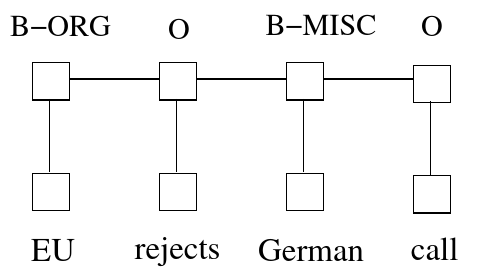
\includegraphics[scale=0.4]{Figures/crf.png}
    \caption{A Linear Chain CRF network}
    \label{fig:crf-net}
\end{figure}


\subsection{BiLSTM-CRF Networks}
NER imposes several dependencies among labels, therefore it would be impossible to model by predicting each label independently. A BiLSTM-CRF Network \cite{lample2016neural} uses a BiLSTM as feature extractor and feeds the features into a CRF layer on top of it to model tagging decisions jointly. The resulting architecture is shown in figure \ref{fig:bilstm-crf-arch}.
For an input sequence $X=(x_1,x_2,..,x_n)$ and a sequence of predictions $Y=(y_1,y_2,...,y_n)$, the predictions' scores are defined as:

\begin{equation}
    s(X,Y) = \sum^n_{i=0} A_{y_i,y_{i+1}} + \sum^n_{i=1} P_{i,y_i}
\end{equation}

\noindent where $P$ is the matrix of scores output by the BiLSTM and $A$ is a matrix of transition scores (essentially bigram compatibility scores) such that $A_{ij}$ represents the score of transitioning from tag $i$ to tag $j$. The score is then transformed into a probability by a softmax function.
During training the log-likelihood of the correct tag sequence is maximized.

In this work I used the same BiLSTM network described in section \ref{sec:lstm}, replacing the Softmax layer with a CRF layer from the pytorch-crf package.

\begin{figure}
    \centering
    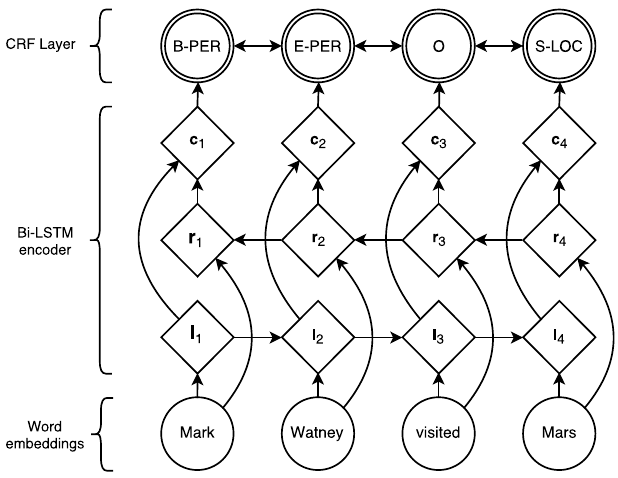
\includegraphics[scale=0.4]{Figures/bilstm-crf.png}
    \caption{BiLSTM-CRF architecture}
    \label{fig:bilstm-crf-arch}
\end{figure}


\section{Training}
The CRF model was trained with the default L-BFGS algorithm, $L_1 + L_2$ regularization and very basic features consisting of a bias set to 1 and the lowercase token string.

Both the BiLSTM and the BiLSTM-CRF networks were trained with the same hyperparameters: batch size of 60, 10 epochs and Adam optimizer with learning rate set to 0.01. The BiLSTM was trained with \texttt{BCELoss}, PyTorch's implementation of Binary Cross Entropy which accepts network scores and one-hot encoded labels directly. The BiLSTM-CRF instead was trained with the CRF layer loss, the negative log-likelihood.


\section{Evaluation}
All three models were evaluated on the test set using a function that removes padding before computing the accuracy score.
As can be calculated from table \ref{tab:conll-distrib}, 88.3\% of tags are Os. Even without padding, the vast majority of tokens in the dataset are Os. This means that models are encouraged to predict O always since it is the most common class and by doing this they can achieve good accuracy while actually not recognizing most entities. 
This is why in NER applications $F_1$ score is preferred to accuracy. So in addition to accuracy I computed the entity-level micro-averaged $F_1$ score using an ad-hoc script provided by the dataset itself. 
Other than comparing the three models of this project between each other, they are compared with three of the most popular and widely used NLP toolkits: Stanza, spaCy and Flair. 
The performances used in the comparison were took from each toolkit respective web pages, where they report the same $F_1$ score used here and can therefore be compared with this work.
The accuracies included in the comparison instead come from spaCy "Fact \& Figures" \cite{spacyfig} web page because the other toolkits don't report them. Keep in mind that:

\begin{itemize}
    \item \cite{spacyfig} reports accuracy for the RoBERTa model but not the $F_1$ score which instead I took from \cite{spacyhugging}. \cite{spacyhugging} does not report the $F_1$ score on RoBERTa, but on the \texttt{en\_core\_web\_trf} pipeline which does include RoBERTa but it might not be the same pipeline used by \cite{spacyfig}.
    \item spaCy doesn't specify if padding was considered while computing accuracy or if it was masked.
\end{itemize}

\noindent The results are shown in table \ref{tab:results}.

% Please add the following required packages to your document preamble:
% \usepackage{booktabs}
\begin{table}
\centering
\begin{tabular}{@{}ccc@{}}
\toprule
\textbf{Model / Toolkit} & \textbf{Accuracy without padding} & \textbf{$F_1$} \\ \midrule
BiLSTM                   & 94.7                              & 73.3           \\
CRF                      & 91.1                              & 62.2           \\
BiLSTM-CRF               & 94.7                              & 75.9           \\
Stanza                   & 92.1*                             & 92.1 \cite{stanzaperf}   \\
Flair                    & 93.1*                             & 94.1 \cite{flair}        \\
spaCy                    & 91.6*                             & 89.9 \cite{spacyhugging} \\ \bottomrule\\
\end{tabular}
\caption{Comparison of this work models, Stanza, Flair and spaCy\\
* = standard accuracy, from \cite{spacyfig}}
\label{tab:results}
\end{table}


\section{Conclusion}

From the results it can be observed that:

\begin{itemize}
    \item In terms of $F_1$ score all three toolkits largely surpass the simpler models.
    \item In terms of accuracy, this work achieves higher scores than the toolkits. However, since I used a very simple model it is really unlikely that it could best the most popular models on the market. For example, the accuracy reported for spaCy is for a Transformer, RoBERTa, which should clearly perform way better than such a simple BiLSTM. This may be a symptom of an error in my code or it could be due to the high number of O tags in the dataset. This could make the accuracy score unreliable. In fact, even achieving higher accuracy, the simpler models achieve much lower $F_1$ score.
    \item Given the simplicity of the model and of the features used, the CRF achieves surprising accuracy and relatively good $F_1$ score, but both are lower than all neural models considered.
    \item The addition of the CRF layer on top of the BiLSTM didn't affect accuracy but improved $F_1$ by 2.6\%.
\end{itemize}


\nocite*
\bibliographystyle{ieeetr}
\bibliography{bib}



% Can use something like this to put references on a page
% by themselves when using endfloat and the captionsoff option.
\ifCLASSOPTIONcaptionsoff
  \newpage
\fi




\end{document}


